\chapter{Week 2 - Global governance and UN environment summits}
\textit{11-09-2017 \\
Henny Romijn}
\section{What did led to the Rio Earth Summit?}
In the 18th century Thomas Malthus was a forerunner. He said: \\
\textit{"The power of population (growth) is indefinitely greater than the power in the earth to produce subsistence for man".} \\
In the 1960s the Flower Power Movement occurs. Following came up some movements in the 60s and 70s like Donenella Meadows "The Limits to Growth" in 1972. In this she describes a long term scenario based on modelling of population growth with a finite resource base. \\
\\
However, it was untill 1972 that the Stockholm Conference on the Human Environment took place. This can be seen as the first attempt at global environmental governance by the United Nations. The focus lay mainly on the western concerns arising from industrialization (e.g. acid rain). There was a strong belief in technofix. Then follows a second oil price hike (1978/79), followed by a world-wide recession, and deepening debt problems for Third World countries. Also around 1980 was the emerging consciousness that environment and development are not separate spheres, and must be addressed together. In 1992 UN Conference on Environment and Development (UNCED): the Rio “Earth Summit” (113 countries, 8000+ delegates, 3000+ NGOs). The Rio Summit was an agreement at the highest level about principles for a global agenda for action: Agenda 21. There was optimism about the willingness to tackle the problems. 

\section{What happened from Rio to Rio+20?}
Accumulating evidence of \textsc{unsustainability}:
\begin{itemize}
\item \textsc{Eco-system degradation};
\item \textsc{Global warming}: if the average global temperature rises by more than two degrees celsius, there will be severe ecological and socio-economic effects;
\item \textsc{Peak oil}: is the point in time when the maximum rate of extraction of petroleum is reached, after which it is expected to enter terminal decline; 
\item \textsc{Inequality}: social inequality is linked to environmental unsustainability for the first time in 2011;
\item \textsc{Urban poverty};
\item \textsc{Food security}: modern, industrial, chemical-intensive agriculture has caused significant ecological degradation, which treatens food security;
\item \textsc{Material flows}: the world urgently needs to seek "decoupling" between economic growth and resource consumption (i.e. "cleantech");
\item \textsc{High debt burdens}: rich countries live beyond their means and want to sustain economic growth. Poor countries suffer from expensive modernization strategies that failed like bank loans; 
\end{itemize}

\section{What are the Millenium Development Goals (MDGs)?}
2000: UN Millenium Declaration. Its conclusion was that insufficient progress had been made towards SD since the Rio Earth Summit in 1992. The Millenium Development Goals were adopted: an agreement by 193 heads of state and 23 international organizations. These goals had to be achieved by 2015. It became subject to controversy over dominance of business interests and market-driven policies for sustainable development. The Millenium Development Goals:
\begin{figure}[ht]
\begin{center}
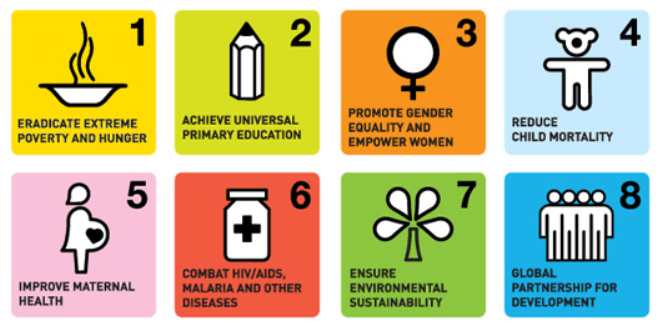
\includegraphics{MDG}
\end{center}
\end{figure}

\clearpage

\section{What are the Sustainable Development Goals (SDGs)?}
The Sustainable Development Goals (abbreviated as SDGs) are a set of 17 global goals with 169 targets among them. Led by the United Nations through a deliberative process involving its 193 Member States, as well as global civil society, the goals are contained in a resolution in the end of 2015. The SDGs were more participative in the design process than the MDGs and there was more balance between development and environment. 

\begin{figure}[ht]
\begin{center}
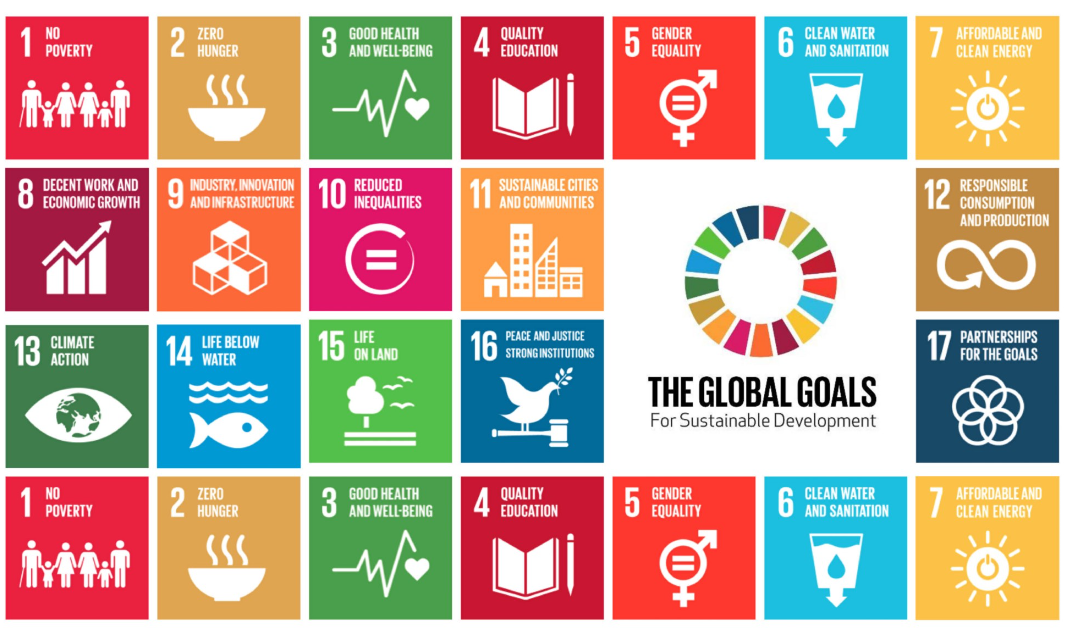
\includegraphics[scale=0.75]{SDG}
\end{center}
\end{figure}

\section{Kyoto: what has been done to sustain further reduction of emmissions?}
The Kyoto Protocol is an international treaty which extends the 1992 United Nations Framework Convention on Climate Change (UNFCCC) that commits State Parties to reduce greenhouse gas emissions, based on the scientific consensus that 
\begin{itemize}
\item global warming is occurring and 
\item it is extremely likely that human-made CO2 emissions have predominantly caused it. 
\end{itemize} 
There are currently 192 parties (Canada withdrew). The Kyoto Protocol implemented the objective of the UNFCCC to fight global warming by reducing greenhouse gas concentrations in the atmosphere to "a level that would prevent dangerous anthropogenic interference with the climate system". The Protocol is based on the principle of common but differentiated responsibilities: it puts the obligation to reduce current emissions on developed countries on the basis that they are historically responsible for the current levels of greenhouse gases in the atmosphere. Kyoto has been much criticized because there is no obligation to join and freedom to quit. Also, the results are limited. Despite all the criticisms, in 2012 Kyoto was extended to 2020 (with 18\% reduction target compared to 1990), because there was no agreement on a follow-up treaty. Finally: Paris agreement (December 2015): new, “improved” UN protocol, due to start in 2020, based on “Intended Nationally Determined Contributions”. But it is still a voluntary agreement.

\clearpage